\input ../SlidePreamble
\input ../preamble


\begin{document}

{\Huge
  \centerline{\bf TTIC 31230,  Fundamentals of Deep Learning}
  \vfill
  \centerline{David McAllester, Autumn   2022}
  \vfill
  \centerline{\bf Contrastive Coding}
  \vfill
  \centerline{\bf Tokenization}
  
  \vfill
  \centerline{\bf Autoregressive Image and Voice Models}
  \vfill
  \vfill

\slide{Contrastive Coding for Speech}
\centerline{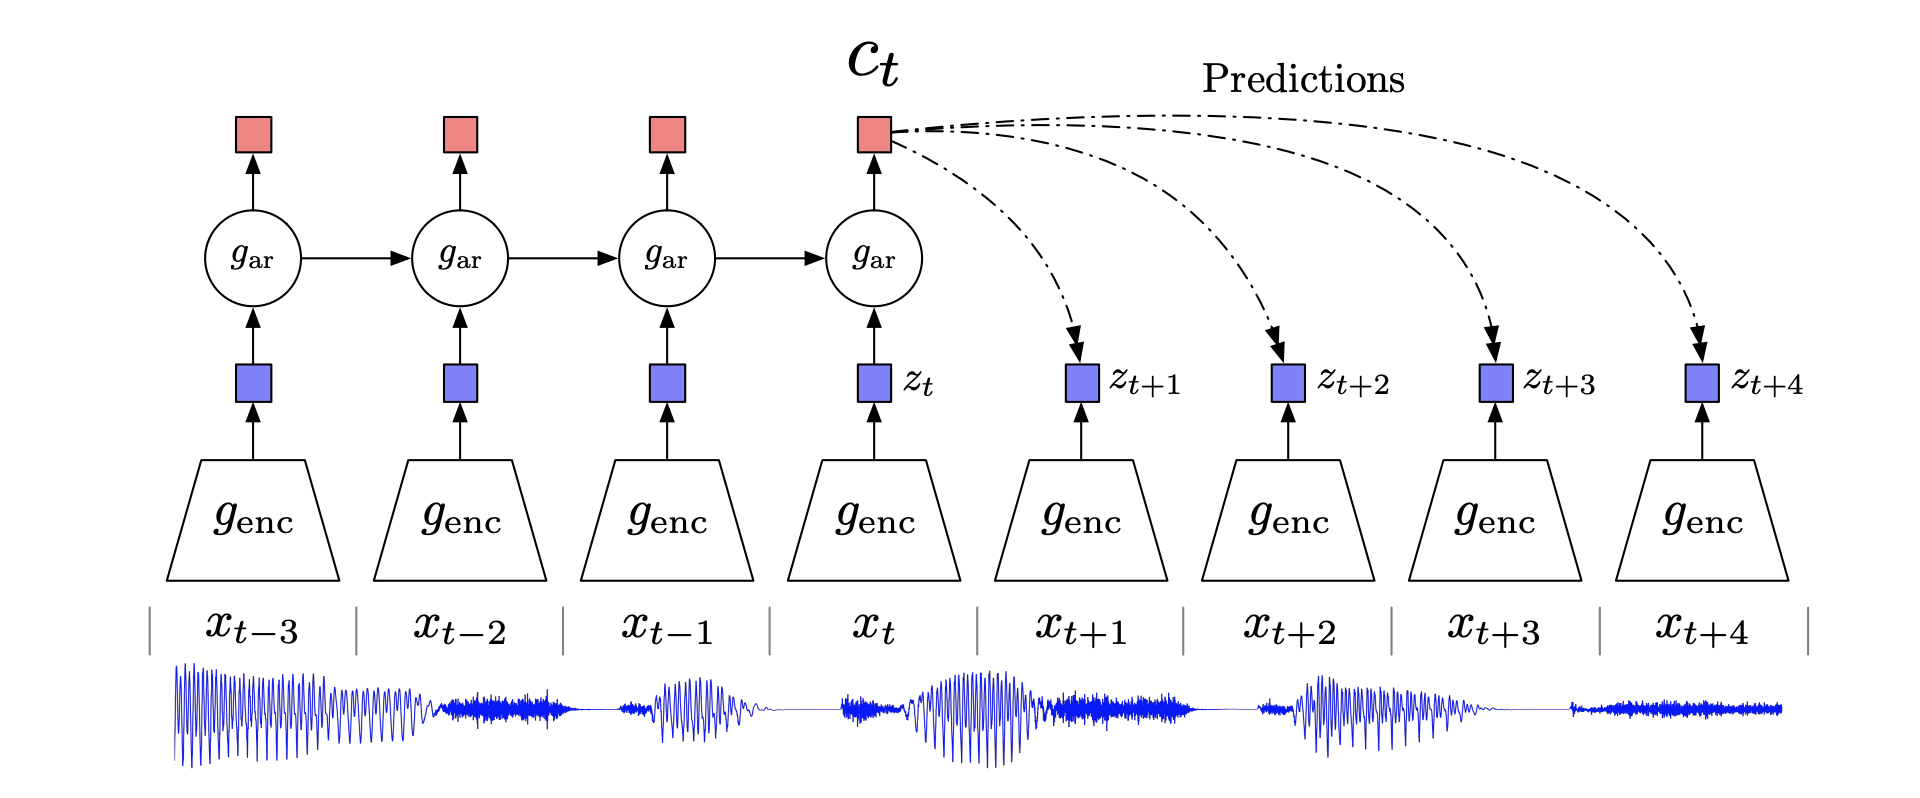
\includegraphics[width = 6 in]{\images/CPC}}
\centerline{\huge van den Oord, Li and Vinyals,}
\centerline{\huge Representation Learning with Contrastive Predictive Coding, 2018}

\vfill
What should we abstract from the past that is relevant to the future?

\slide{Contrastive Coding for Speech}
\centerline{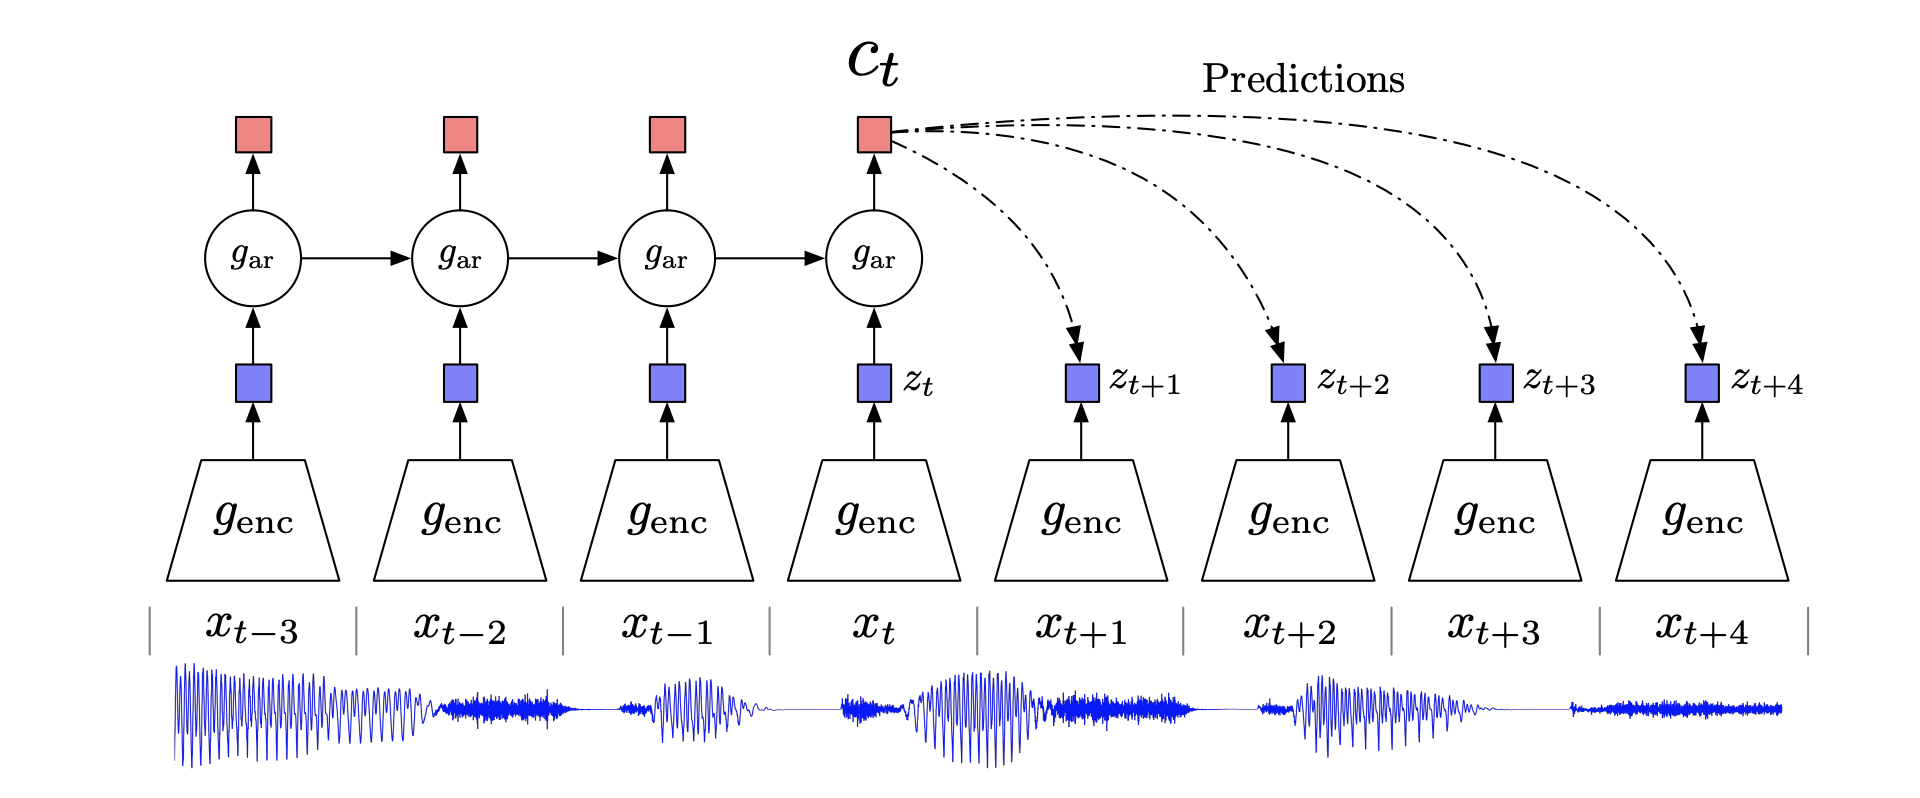
\includegraphics[width = 6 in]{\images/CPC}}

\vfill
{\bf Unlike VAEs}, contrastive coding is about {\bf capturing mutual information}.
Intuitively we want to {\bf separate signal from noise} and avoid modeling noise.

\slide{Contrastive Coding for Speech}
\centerline{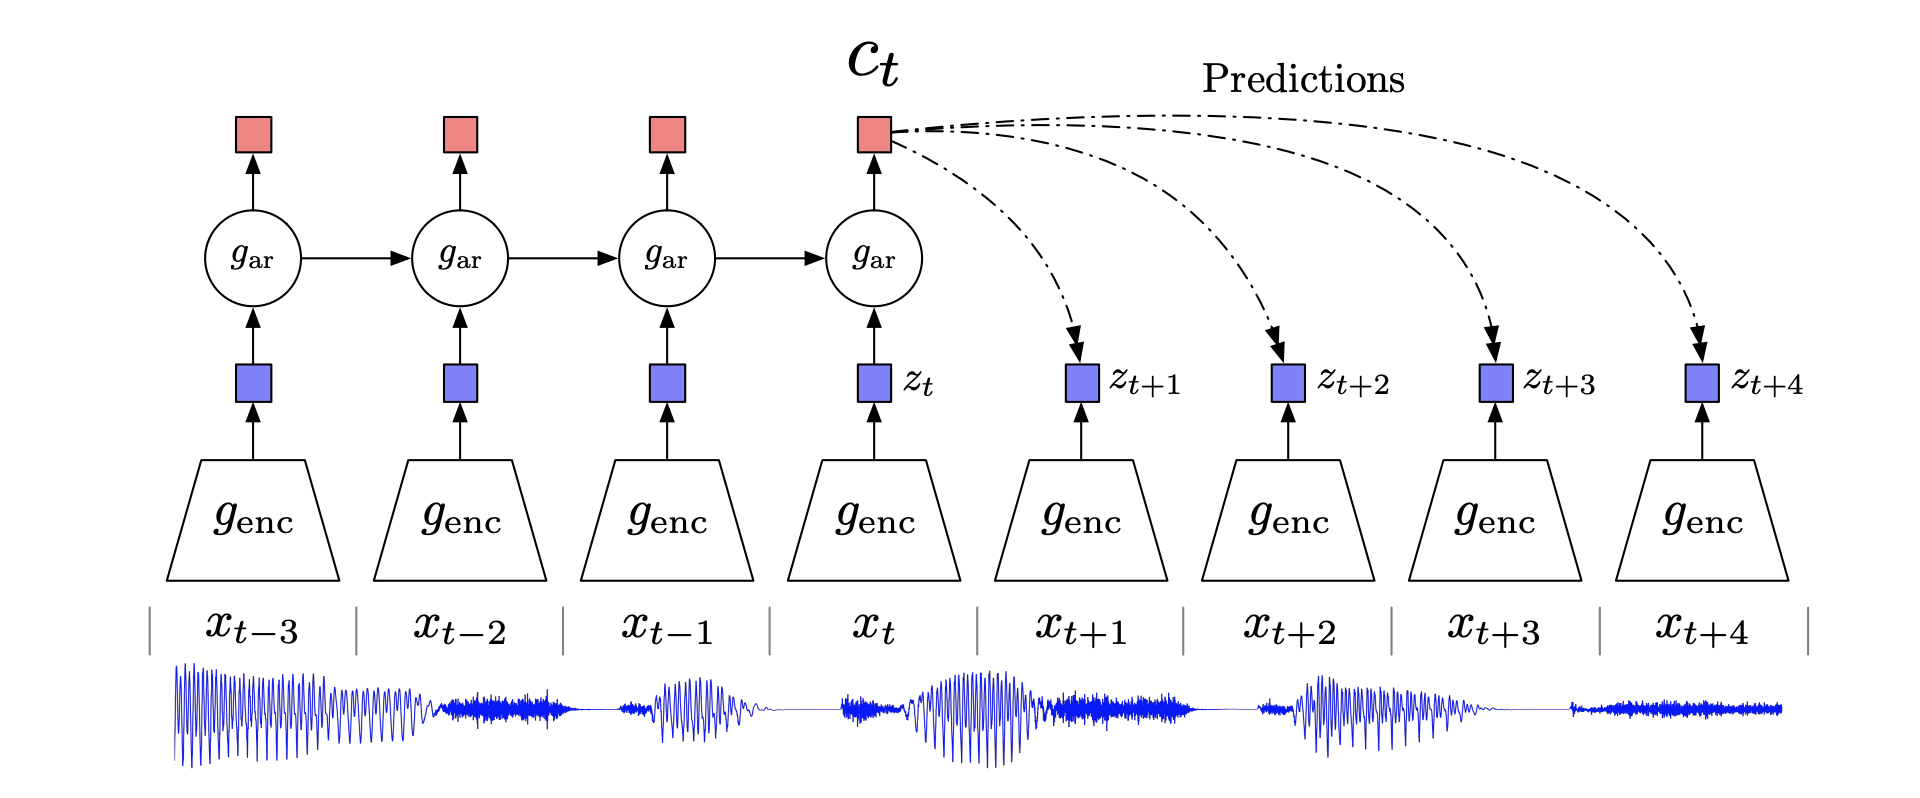
\includegraphics[width = 6 in]{\images/CPC}}

\vfill
We abstract this problem to that of capturing the mutual information between any two arbitrary random variables $x$ and $y$.

\slide{Contrastive Coding}

 We consider a population distribution on pairs $(x,y)$.
 
 \vfill
 For example:
 
 \vfill
\begin{itemize}
\item $x$ might be an image and $y$ might be the text of a caption for image $x$ (CLIP).

\vfill
\item $x$ might be an video frame and $y$ video frame a second later.

\vfill
\item $x$ might be a window of a sound wave and $y$ a later window (Wav2Vec).

\vfill
\item $x = f(z)$ and $y = f(z)$ where $f$ and $g$ are transformation functions on an image $z$ such as  translation, rotation, color shift, or cropping. (augmentation) of $x$. (SimCLR)
\end{itemize}

\slide{Contrastive Coding}

We draw pairs $(x_1,y_1), \ldots (x_B,y_B)$ from the population.
We then select $b$ uniformly from $1$ to $B$ and construct the tuple $(x_b,y_1,\ldots,y_B,b)$.

\vfill
We then train a model to predict $b$.
\vfill
{\huge
\begin{eqnarray*}
\enc_x^*,\enc_y^* & = & \argmin_{\enc_x,\enc_y} \;E_{(x,y_1,\ldots,y_B,b)}\left[-\ln P_{\enc_x,\enc_y}(b|x,y_1,\ldots,y_B)\right]
\end{eqnarray*}

\begin{eqnarray*}
P_{\enc_x,\enc_y}(b|x,y_1,\ldots,y_B) & = & \softmax_b\; \enc_x(x)^\top\enc_y(y_b)
\end{eqnarray*}
}

\slide{The Contrastive Coding Theorem}

For any distribution on pairs $(x,y)$, with contrastive probabilities computed by

\begin{eqnarray*}
P(b|x,y_1,\ldots,y_B) & = & \softmax_b\;s(x,y_b)
\end{eqnarray*}

we have

{\huge
\begin{eqnarray*}
I(x,y) & \geq & \ln B - \;\;E_{(x,y_1,\ldots,y_B,b)}\left[-\ln P(b|(x,y_1,\ldots,y_B))\right]
\end{eqnarray*}
}

Chen et al., On Variational Bounds of Mutual Information, May 2019.

\slide{CLIP, January 2021, OpenAI}

CLIP: Contrastive Language-Image Pre-training.

\vfill
Trained on images and associated text (such as image captions or hypertext links to images) CLIP computes embeddings of text and embeddings of images
(``co-embeddings'') trained to capture the mutual information between the two.

\slide{CLIP Constrastive Coding}

\centerline{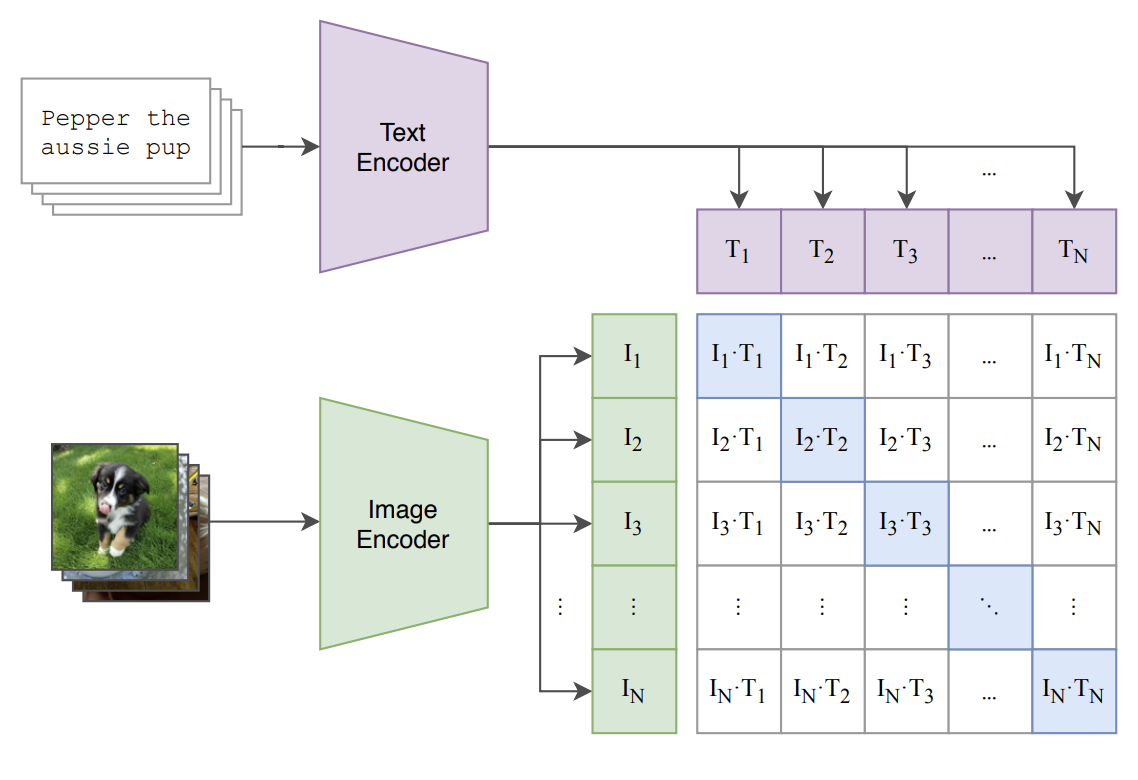
\includegraphics[height= 5in]{\images/CLIPTraining}}

\slide{CLIP Image Classification}

\centerline{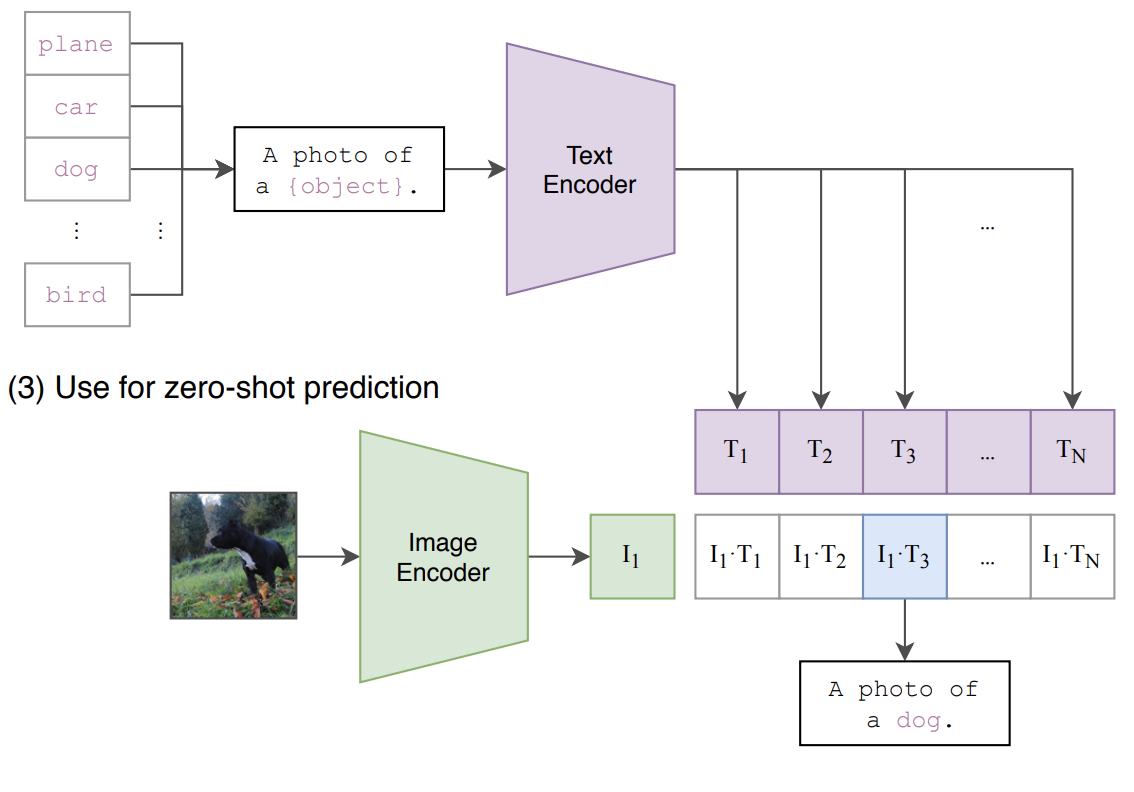
\includegraphics[height= 5in]{\images/CLIPClassifier}}

\slide{Zero-Shot Image Classification}

\centerline{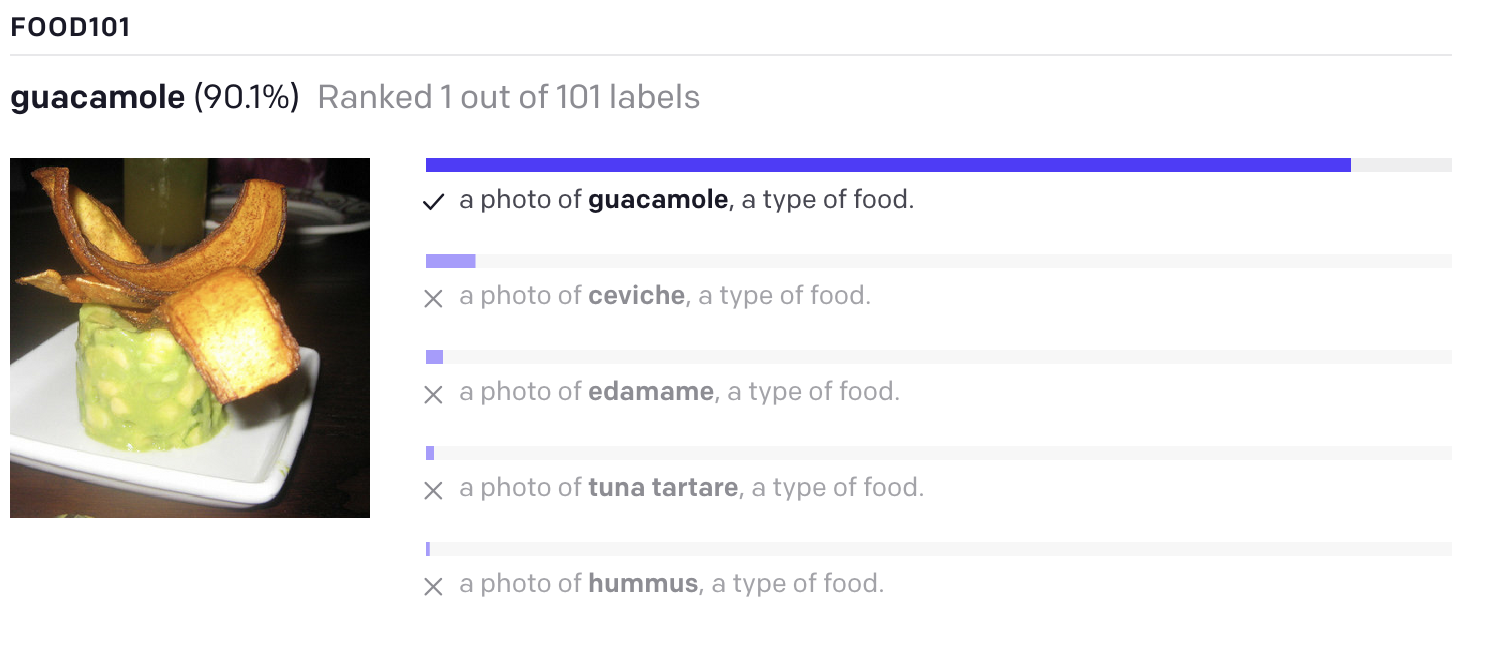
\includegraphics[width = 7in]{\images/CLIP0}}

\slide{Zero-Shot Image Classification}

\centerline{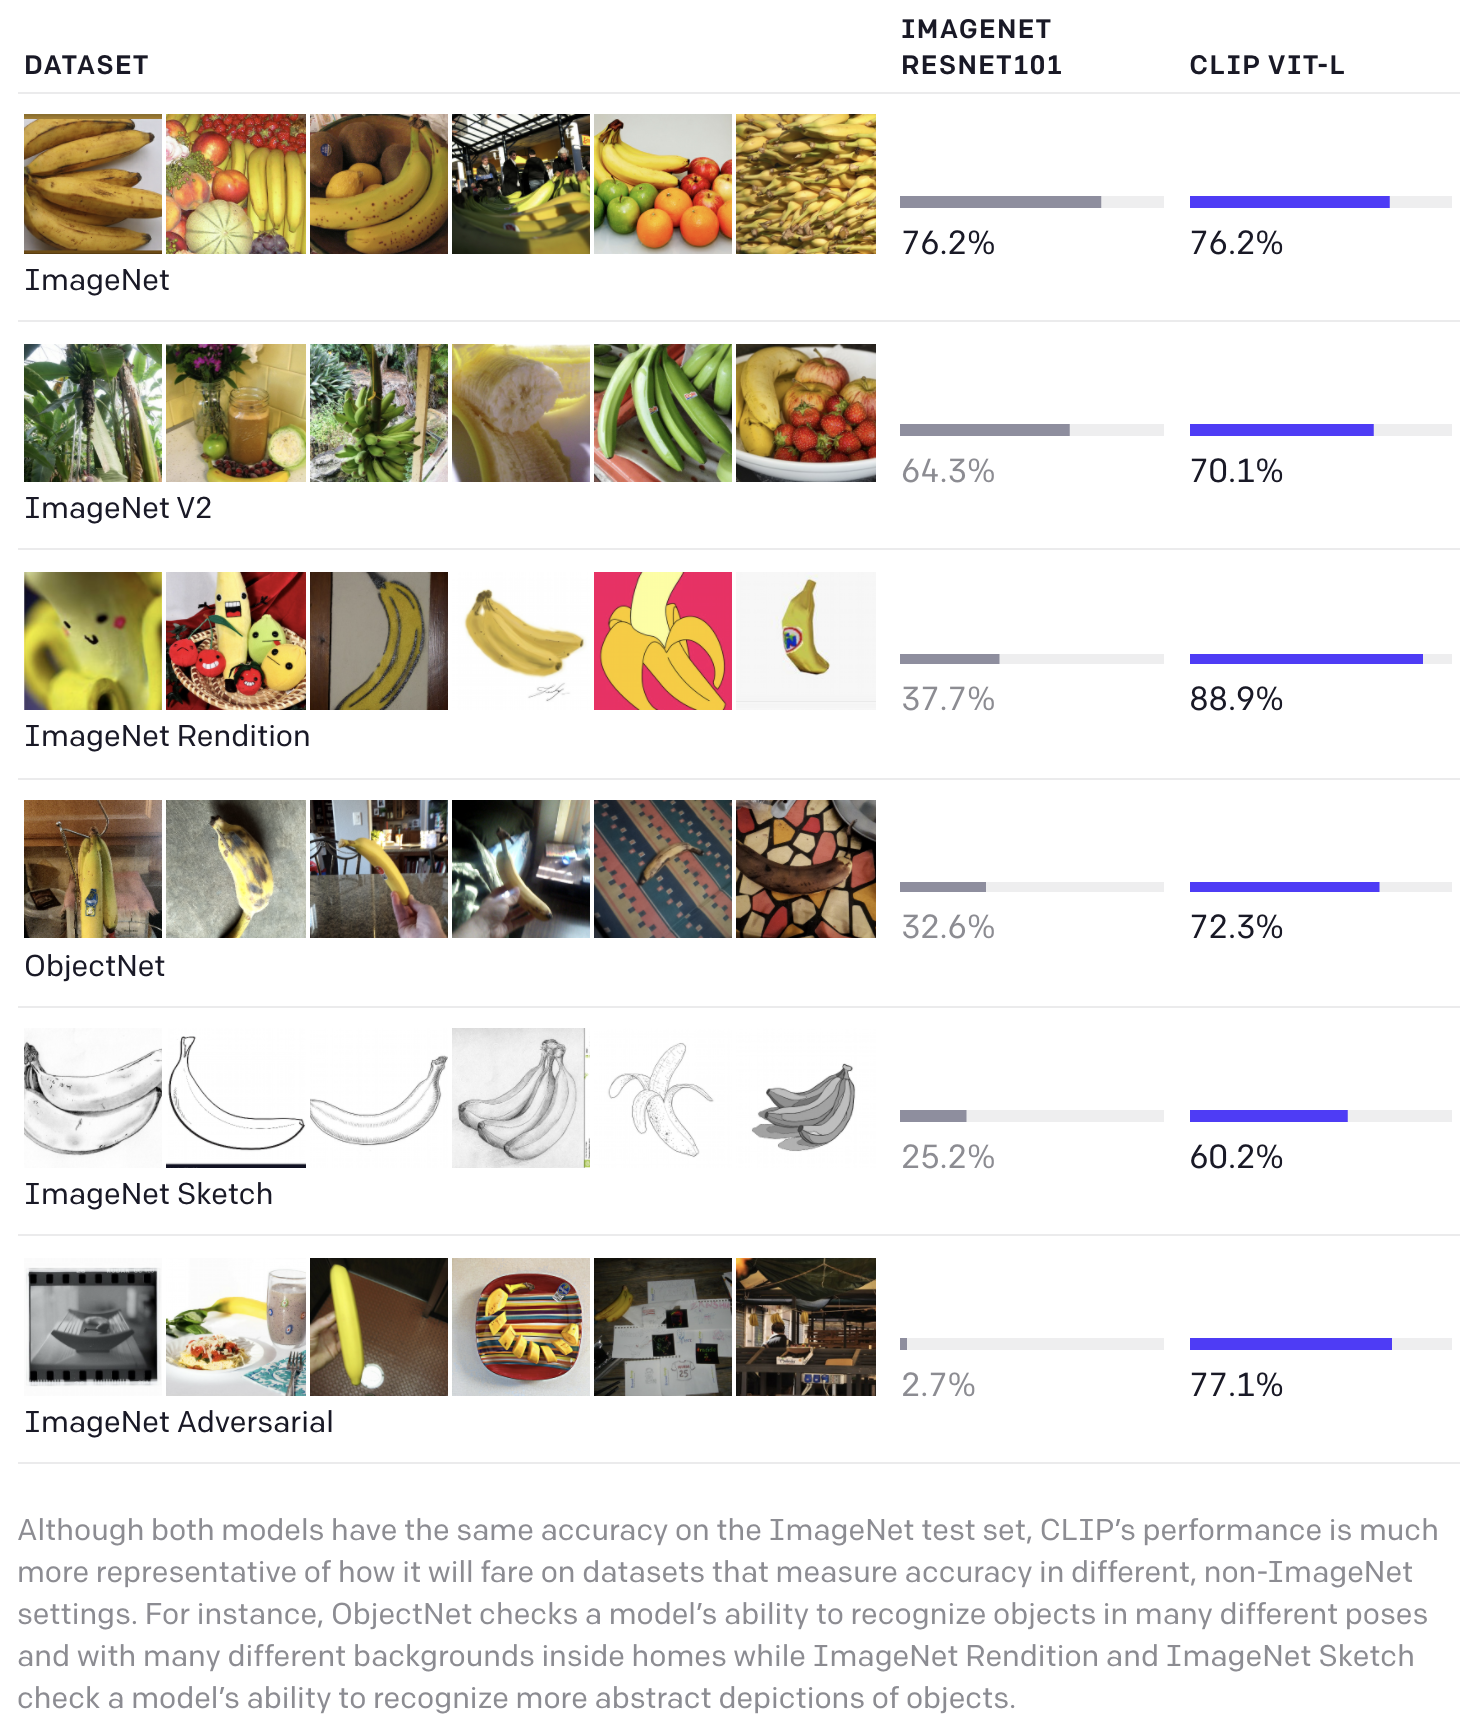
\includegraphics[height= 5in]{\images/CLIP1}}

\slide{A Weakness of Contrastive Coding}

{\huge
\begin{eqnarray*}
I(x,y) & \geq & \ln B - \;\;E_{(x,y_1,\ldots,y_B,b)}\left[-\ln P(b|(x,y_1,\ldots,y_B)\right]
\end{eqnarray*}
}

The discrimination problem may be too easy.

\vfill
The guarantee can never be stronger than $\ln B$ where $B$ is the batch size.

\vfill
Suppose we have 100 bits of mutual information as seem plausible for translation pairs.

\slide{Addresses the Weakness with Large Batch Size}

\begin{eqnarray*}
I(x,y) & \geq & \ln B - \;\;E_{(x,y_1,\ldots,y_B,b)}\left[-\ln P(b|(x,y_1,\ldots,y_B)\right]
\end{eqnarray*}

\vfill
For CLIP the batch size $B = 2^{15}$ so we can potentially guarantee 15 bits of mutual information.

\slide{Wav2vec 2.0, June 2020, Facebook}

\vfill
Trained on 53k hours of unlabeled audio (no text) they convert speech to a sequence of discrete quantized vectors they call ``pseudo-text units''.

\vfill
By training on only one hour of human-transcribed audio, and using the Wav2vec transcription into pseudo-text, they outperform the previous state of the
art in word error rate for 100 hours of human-transcribed text.

\slide{Autoregressive Image and Voice Modeling}

Strong VAE image modeling was first achieved autoregressive image modeling.

\vfill
\centerline{van den Oord, Vinyals and Kavukcuoglu,}
\centerline{Neural Discrete Representation Learning, {\bf 2017}}

\vfill
\centerline{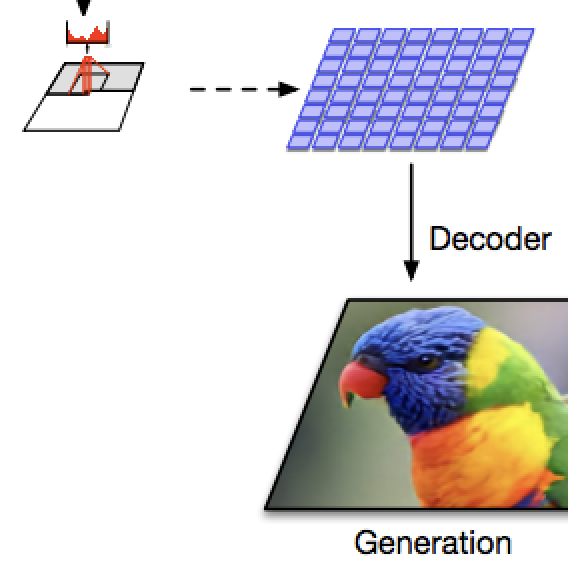
\includegraphics[height = 2in]{\images/VQ-OneLayer} 
\parbox[b]{2.5in}{\huge Token Transformer \\ \\ \\ \\ Tokens-to-Image \\~}}

\slide{VQ-VAE-2, June 2019}

\centerline{Generating Diverse High-Fidelity Images
with VQ-VAE-2}

\vfill
\centerline{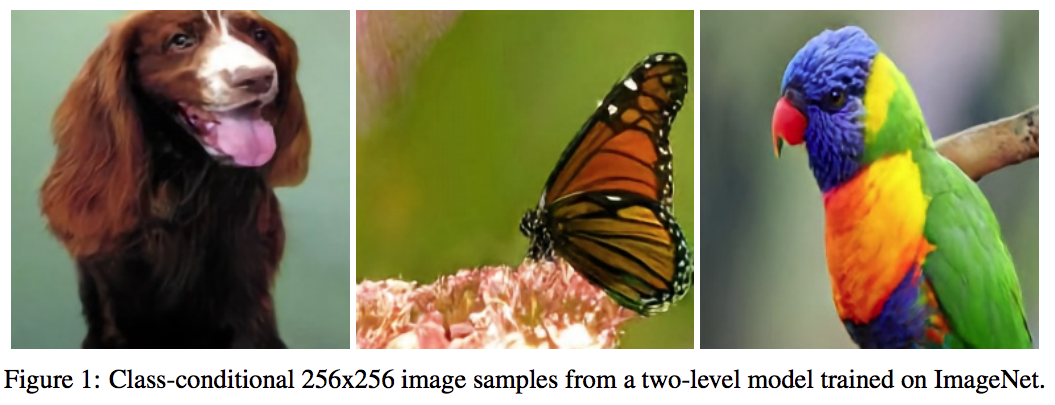
\includegraphics[width = 8in]{\images/VQ-VAE21}}


\slide{DALLE-1, January 2021}

\vfill
\centerline{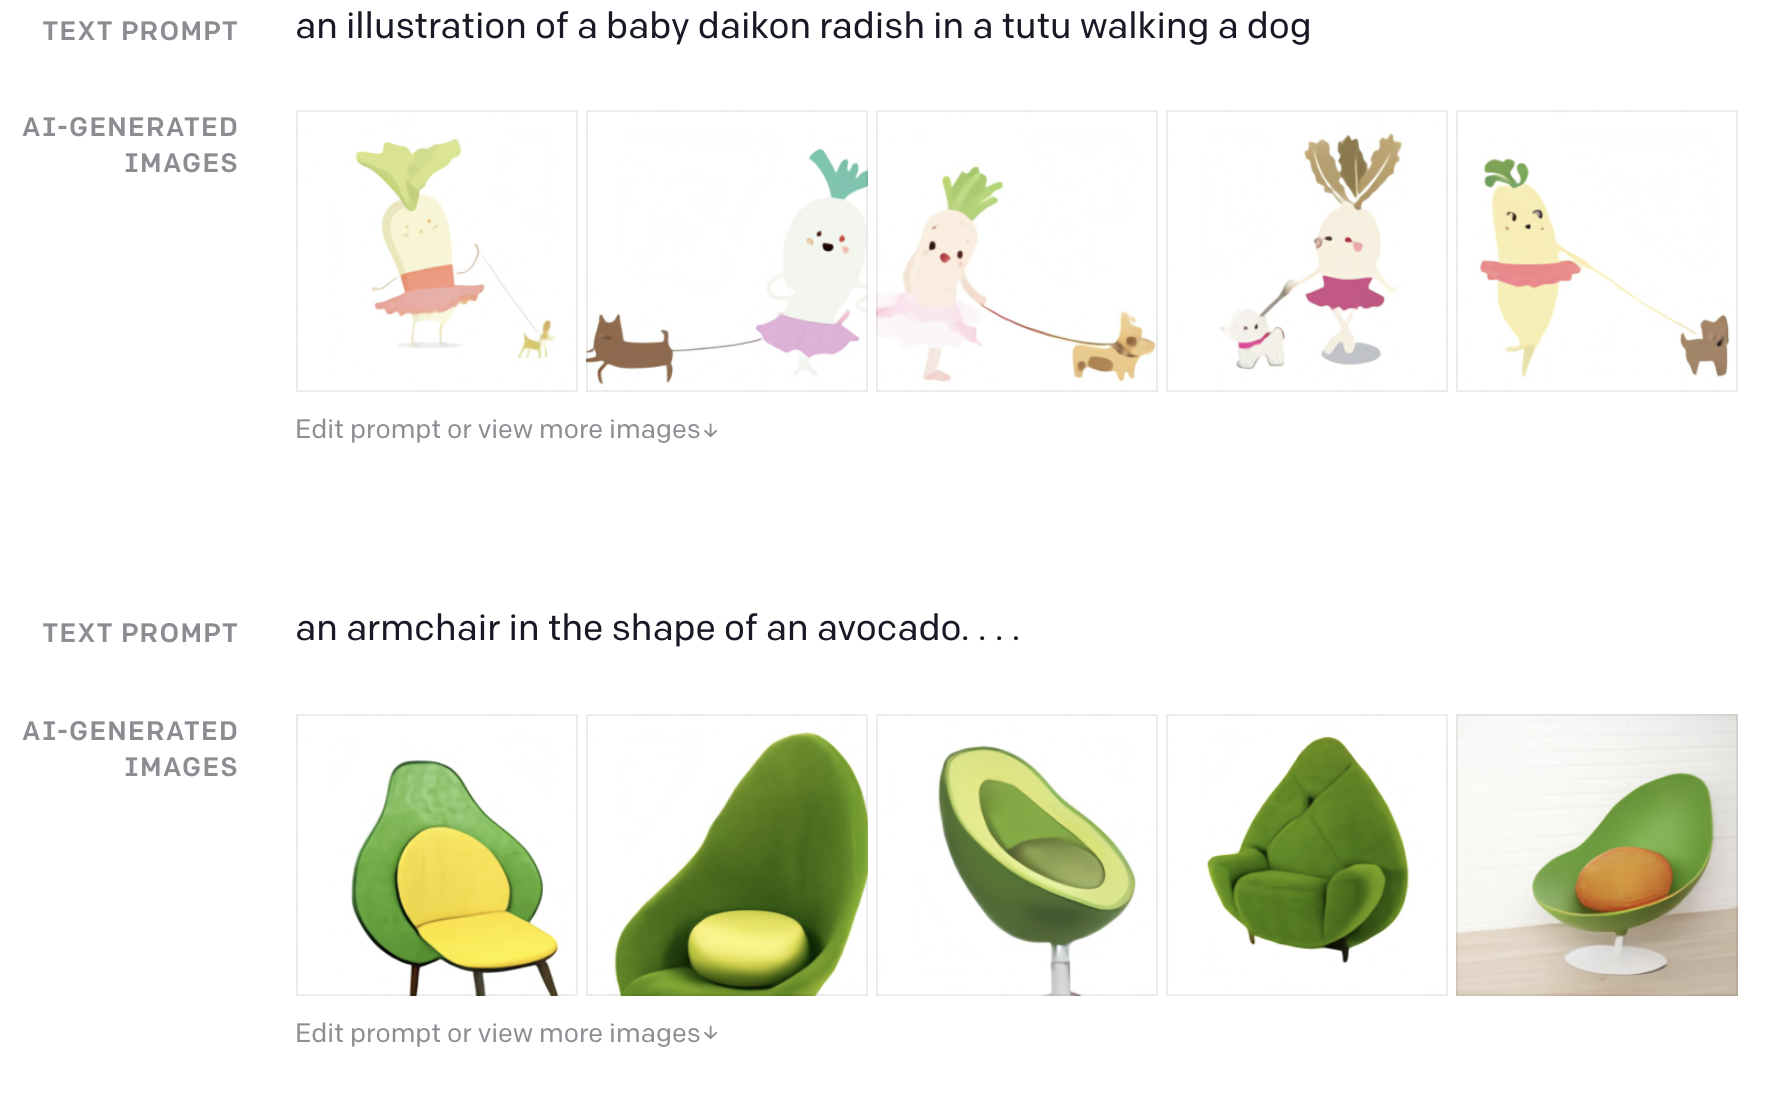
\includegraphics[width = 8in]{\images/DALLE1}}

\slide{Parti, June 2022}

\centerline{\huge Scaling Autoregressive Models for Content-Rich Text-to-Image Generation}
\centerline{\huge Yu et al.}

\vfill
\centerline{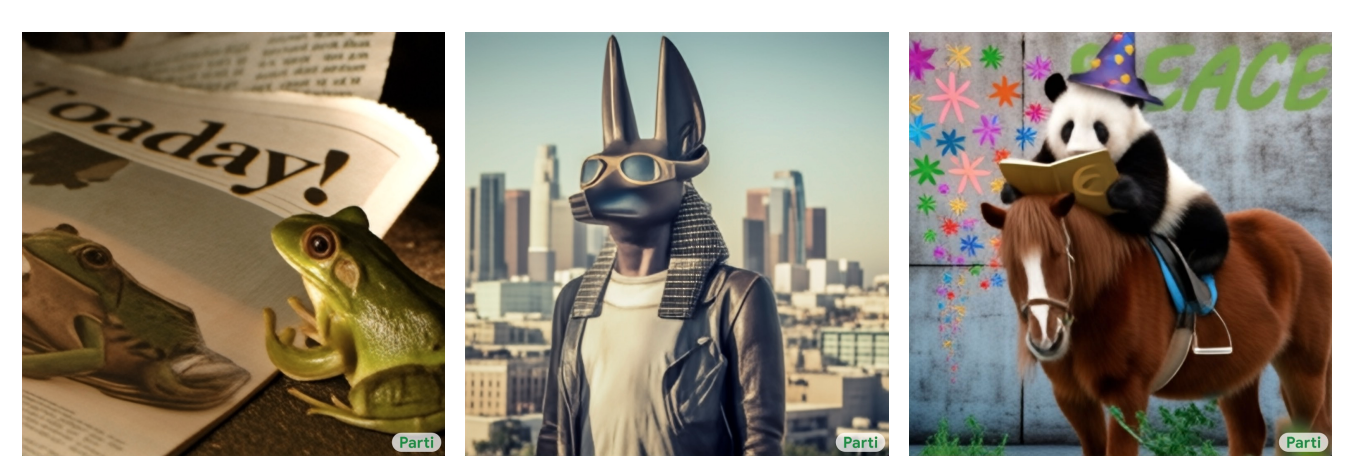
\includegraphics[width = 9in]{\images/Parti}}


\slide{CM3Leon, September 2023}

\centerline{\Large Scaling Autoregressive Multi-Modal Models: Pretraining and Instruction Tuning}
\centerline{\Large Yu et al.}

\vfill
\centerline{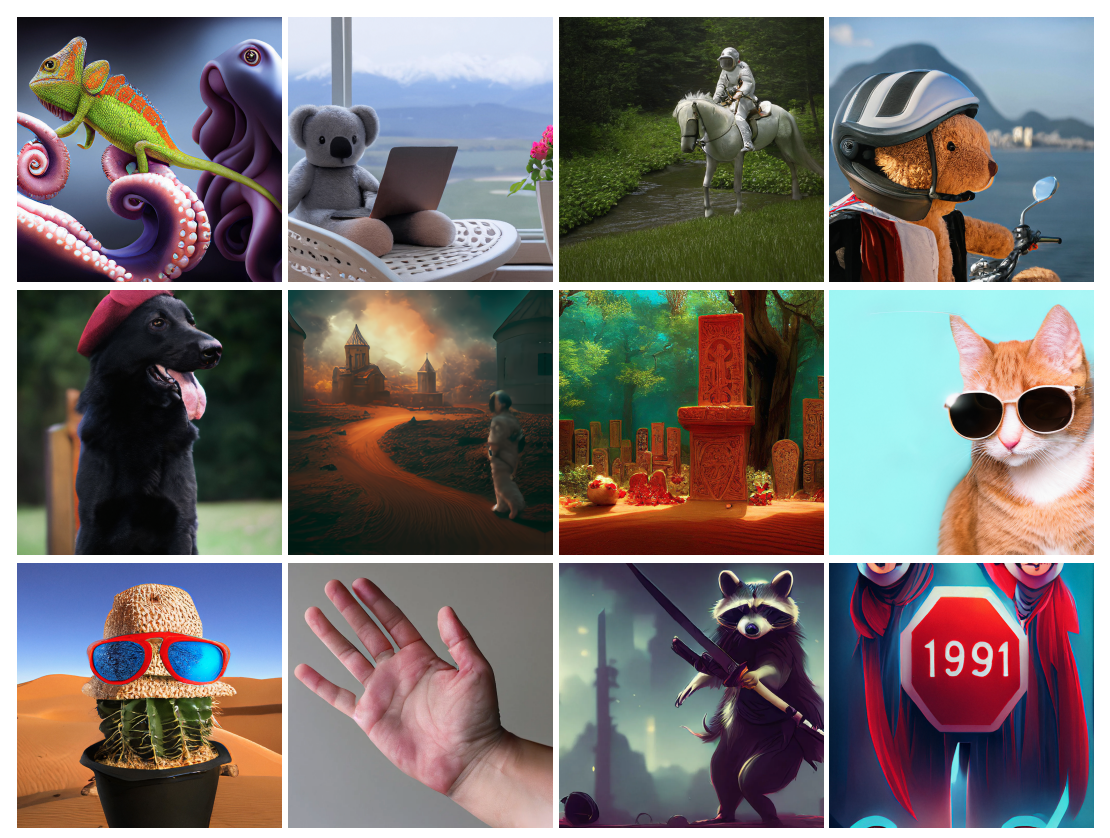
\includegraphics[width = 5.7in]{\images/CM3Leon}}

\slide{GLSM, February 2021, Facebook}

Generative Spoken Language Model (GSLM)

\vfill
They then train a generative model of the sequences of pseudo-text units learned from unlabeled audio.


\vfill
This model can continue speech from a speech prompt in much the same way that GPT-3 continues text from a text prompt.

\vfill
Semantic and grammatical structure in a ``unit language model'' is recovered
from speech alone.

\slide{Voice-Text Language Model (VoxtLM), September 2023}

This is similar to CM3Leon but for voice and text rather than images and text.

\vfill
Voice is tokenized and then a transformer is used to model sequences that alternate voice and text.

\slide{Tokenization of Images and Voice}

\centerline{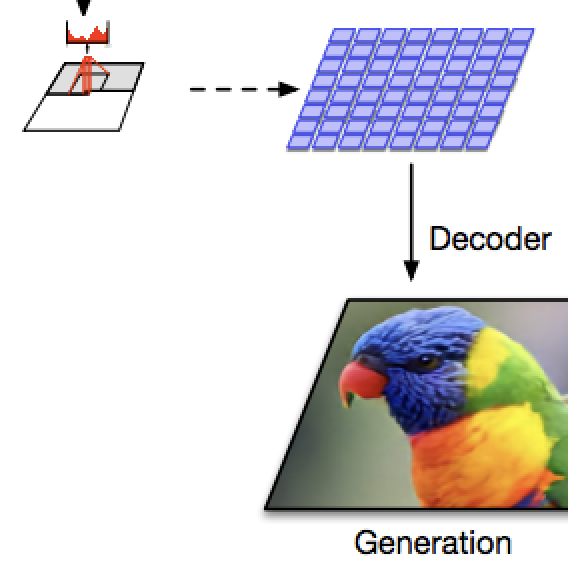
\includegraphics[height = 2in]{\images/VQ-OneLayer} 
\parbox[b]{2.5in}{\huge Token Transformer \\ \\ \\ \\ Tokens-to-Image \\~}}

\vfill
Let $y$ range over a population (such as images or sound waves).

\vfill
Assume that a given $y$ is encoded as a tensor denoted {\color{red} $z_{\enc,p}(y)$} where $p$ is a ``position in $y$'' (a pixel in an image tensor
or time window in a sound tensor) and {\color{red} $z_{\enc, p}(y) \in R^d$} is a vector.

\slide{Vector Quantization (Tokenization)}

\centerline{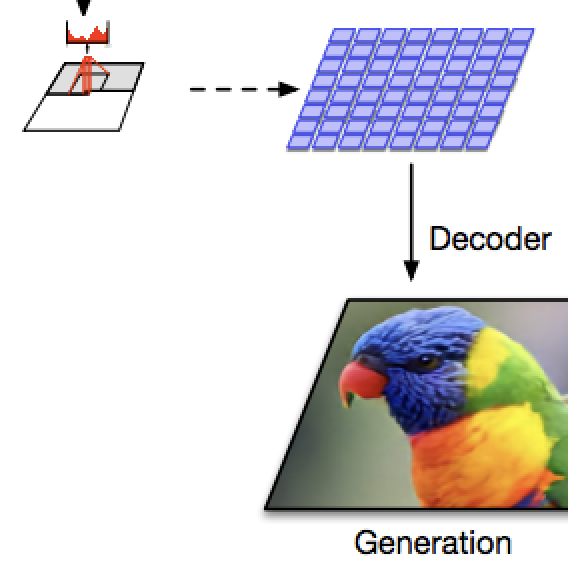
\includegraphics[height = 2in]{\images/VQ-OneLayer} 
\parbox[b]{2.5in}{\huge Token Transformer \\ \\ \\ \\ Tokens-to-Image \\~}}

\vfill
Assume a finite set of $K$ ``tokens'' where token $k$ has an embedding vector $e(k) \in R^d$.

\vfill
Define $k_{\enc,p}(y)$ by
$$k_{\enc,p}(y)= \argmin_k\;\frac{1}{2}||z_{\enc,p}(y)-e(k)||^2$$

\slide{Reconstruction Loss}

\centerline{\parbox[b]{1.0in}{\huge $P_\pri(k)$ \\ \\ \\ \\ \\ ~}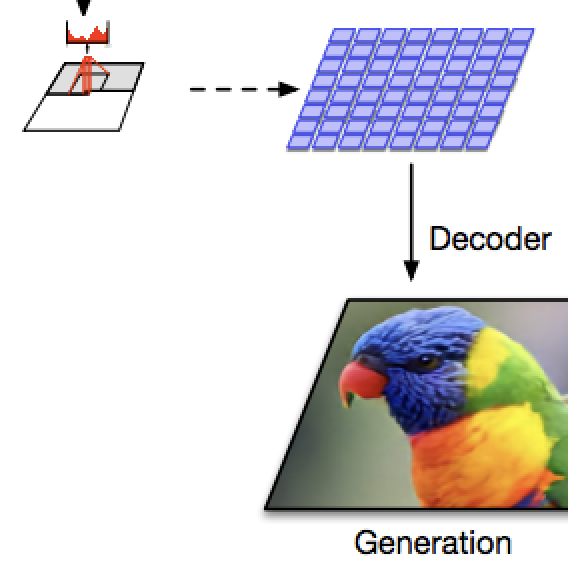
\includegraphics[height = 2in]{\images/VQ-OneLayer} 
\parbox[b]{2.5in}{\huge $k_\enc(y)$ \\ \\ \\ \\ $y$ \\~}}

We now have a VAE where the tensor $k_\enc(y)$ is the latent variable.

\vfill
The encoder and decoder are trained jointly.

\vfill
The prior is a transformer trained after the encoder and decoder are fully trained.

\slide{Training the Encoder and Decoder}
\centerline{\parbox[b]{1.0in}{\huge $P_\pri(k)$ \\ \\ \\ \\ \\ ~}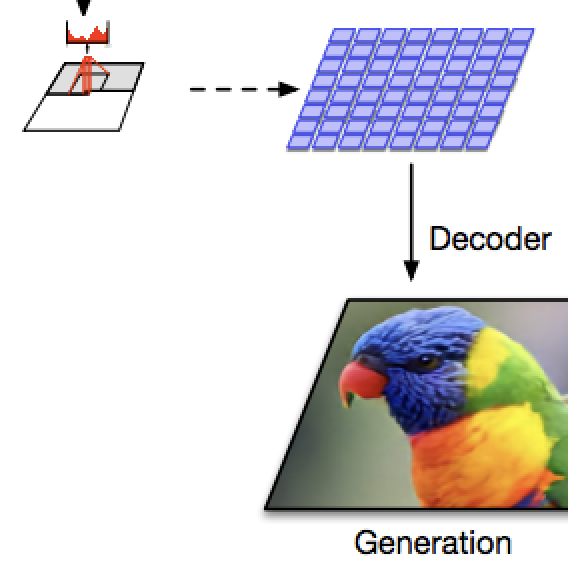
\includegraphics[height = 2in]{\images/VQ-OneLayer} 
\parbox[b]{2.5in}{\huge $k(z_\enc(y))$ \\ \\ \\ \\ $y$ \\~}}

\vfill
Taking $P_\dec(y|k)$ to be ${\cal N}(\hat{y}_\dec(k),I)$ we get an $L_2$ reconstruction loss.

\vfill
$${\cal L}_{\mathrm{Rec}} = \frac{1}{2}||\;y - \hat{y}_\dec(e(k(z_\enc(y))))\;||^2$$

\slide{Training the Encoder and Decoder}
\centerline{\parbox[b]{1.0in}{\huge $P_\pri(k)$ \\ \\ \\ \\ \\ ~}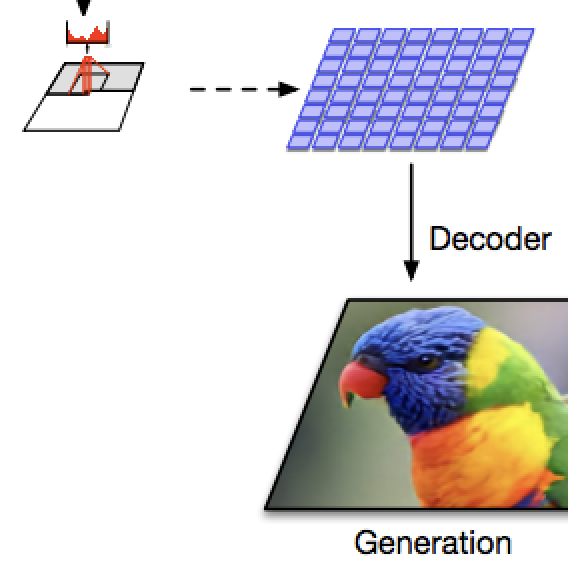
\includegraphics[height = 2in]{\images/VQ-OneLayer} 
\parbox[b]{2.5in}{\huge $k(z_\enc(y))$ \\ \\ \\ \\ $y$ \\~}}

\vfill
$${\cal L}_{\mathrm{Rec}} = \frac{1}{2}||\;y - \hat{y}_\dec(e(k(z_\enc(y))))\;||^2$$

\vfill
Because the tokens are discrete we do not get any gradient on $z_\enc(y)$.

\slide{Straight-Through Gradients}
\centerline{\parbox[b]{1.0in}{\huge $P_\pri(k)$ \\ \\ \\ \\ \\ ~}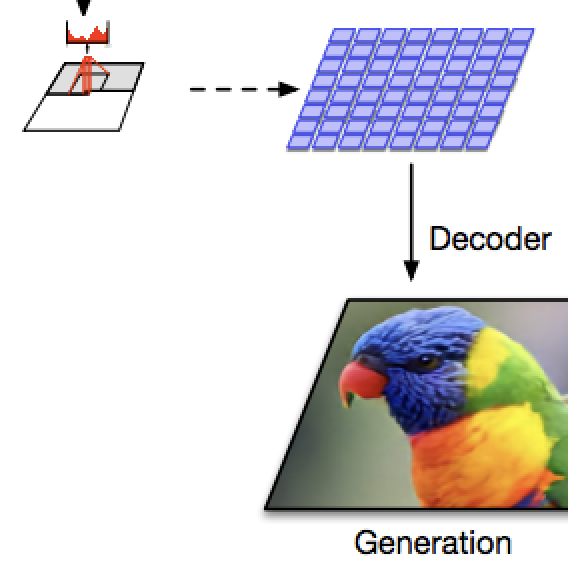
\includegraphics[height = 2in]{\images/VQ-OneLayer} 
\parbox[b]{2.5in}{\huge $k(z_\enc(y))$ \\ \\ \\ \\ $y$ \\~}}

\vfill
$${\cal L}_{\mathrm{Rec}} = \frac{1}{2}||\;y - \hat{y}_\dec(e(k(z_\enc(y))))\;||^2$$

\vfill{
$$z_{\enc,p}(y).\grad = \nabla_{e(k(z_{\enc,p}(y)))} {\cal L}_{\mathrm{Rec}}$$

\slide{K-Means Gradients}

We train $z_\enc(y)$ and the token embeddings $e(k)$.

\vfill
$${\cal L}_{\mathrm{Rec}} = \frac{1}{2}||\;y - \hat{y}_\dec(e(k(z_\enc(y))))\;||^2$$

\vfill{
$$z_{\enc,p}(y).\grad = \nabla_{e(k(z_{\enc,p}(y)))} {\cal L}_{\mathrm{Rec}}$$

\vfill
$${\cal L}_{\mathrm{KM}} = \frac{1}{2}||z_{\enc,p}(y) - e(k(z_{\enc,p}))||^2$$

\vfill{
$$e(k(z_{\enc,p}(y))).\grad \;\pluseq\; \beta \nabla_{e(k(z_{\enc,p}(y)))} {\cal L}_{\mathrm{KM}}$$

\vfill
$\beta$ is a hyper-parameter that adjust the relative learning rates.

\slide{Transformer Training}

Finally we hold the encoder fixed and train the prior $P_\pri(z)$ to be an auto-regressive model of the symbolic image $k_\enc(s)[X,Y]$.

\vfill
\centerline{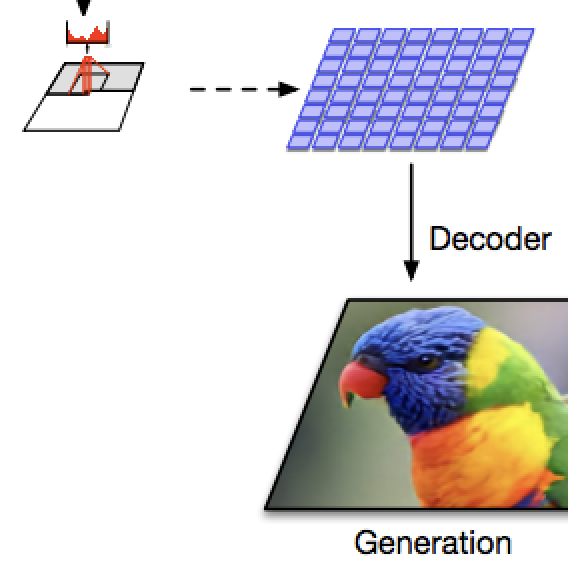
\includegraphics[height = 2in]{\images/VQ-OneLayer}}



\slide{END}

}
\end{document}

